\documentclass{article}
\usepackage{iclr2026_conference,times}

%%%%% NEW MATH DEFINITIONS %%%%%

\usepackage{amsmath,amsfonts,bm}

% Mark sections of captions for referring to divisions of figures
\newcommand{\figleft}{{\em (Left)}}
\newcommand{\figcenter}{{\em (Center)}}
\newcommand{\figright}{{\em (Right)}}
\newcommand{\figtop}{{\em (Top)}}
\newcommand{\figbottom}{{\em (Bottom)}}
\newcommand{\captiona}{{\em (a)}}
\newcommand{\captionb}{{\em (b)}}
\newcommand{\captionc}{{\em (c)}}
\newcommand{\captiond}{{\em (d)}}

% Highlight a newly defined term
\newcommand{\newterm}[1]{{\bf #1}}


% Figure reference, lower-case.
\def\figref#1{figure~\ref{#1}}
% Figure reference, capital. For start of sentence
\def\Figref#1{Figure~\ref{#1}}
\def\twofigref#1#2{figures \ref{#1} and \ref{#2}}
\def\quadfigref#1#2#3#4{figures \ref{#1}, \ref{#2}, \ref{#3} and \ref{#4}}
% Section reference, lower-case.
\def\secref#1{section~\ref{#1}}
% Section reference, capital.
\def\Secref#1{Section~\ref{#1}}
% Reference to two sections.
\def\twosecrefs#1#2{sections \ref{#1} and \ref{#2}}
% Reference to three sections.
\def\secrefs#1#2#3{sections \ref{#1}, \ref{#2} and \ref{#3}}
% Reference to an equation, lower-case.
\def\eqref#1{equation~\ref{#1}}
% Reference to an equation, upper case
\def\Eqref#1{Equation~\ref{#1}}
% A raw reference to an equation---avoid using if possible
\def\plaineqref#1{\ref{#1}}
% Reference to a chapter, lower-case.
\def\chapref#1{chapter~\ref{#1}}
% Reference to an equation, upper case.
\def\Chapref#1{Chapter~\ref{#1}}
% Reference to a range of chapters
\def\rangechapref#1#2{chapters\ref{#1}--\ref{#2}}
% Reference to an algorithm, lower-case.
\def\algref#1{algorithm~\ref{#1}}
% Reference to an algorithm, upper case.
\def\Algref#1{Algorithm~\ref{#1}}
\def\twoalgref#1#2{algorithms \ref{#1} and \ref{#2}}
\def\Twoalgref#1#2{Algorithms \ref{#1} and \ref{#2}}
% Reference to a part, lower case
\def\partref#1{part~\ref{#1}}
% Reference to a part, upper case
\def\Partref#1{Part~\ref{#1}}
\def\twopartref#1#2{parts \ref{#1} and \ref{#2}}

\def\ceil#1{\lceil #1 \rceil}
\def\floor#1{\lfloor #1 \rfloor}
\def\1{\bm{1}}
\newcommand{\train}{\mathcal{D}}
\newcommand{\valid}{\mathcal{D_{\mathrm{valid}}}}
\newcommand{\test}{\mathcal{D_{\mathrm{test}}}}

\def\eps{{\epsilon}}


% Random variables
\def\reta{{\textnormal{$\eta$}}}
\def\ra{{\textnormal{a}}}
\def\rb{{\textnormal{b}}}
\def\rc{{\textnormal{c}}}
\def\rd{{\textnormal{d}}}
\def\re{{\textnormal{e}}}
\def\rf{{\textnormal{f}}}
\def\rg{{\textnormal{g}}}
\def\rh{{\textnormal{h}}}
\def\ri{{\textnormal{i}}}
\def\rj{{\textnormal{j}}}
\def\rk{{\textnormal{k}}}
\def\rl{{\textnormal{l}}}
% rm is already a command, just don't name any random variables m
\def\rn{{\textnormal{n}}}
\def\ro{{\textnormal{o}}}
\def\rp{{\textnormal{p}}}
\def\rq{{\textnormal{q}}}
\def\rr{{\textnormal{r}}}
\def\rs{{\textnormal{s}}}
\def\rt{{\textnormal{t}}}
\def\ru{{\textnormal{u}}}
\def\rv{{\textnormal{v}}}
\def\rw{{\textnormal{w}}}
\def\rx{{\textnormal{x}}}
\def\ry{{\textnormal{y}}}
\def\rz{{\textnormal{z}}}

% Random vectors
\def\rvepsilon{{\mathbf{\epsilon}}}
\def\rvtheta{{\mathbf{\theta}}}
\def\rva{{\mathbf{a}}}
\def\rvb{{\mathbf{b}}}
\def\rvc{{\mathbf{c}}}
\def\rvd{{\mathbf{d}}}
\def\rve{{\mathbf{e}}}
\def\rvf{{\mathbf{f}}}
\def\rvg{{\mathbf{g}}}
\def\rvh{{\mathbf{h}}}
\def\rvu{{\mathbf{i}}}
\def\rvj{{\mathbf{j}}}
\def\rvk{{\mathbf{k}}}
\def\rvl{{\mathbf{l}}}
\def\rvm{{\mathbf{m}}}
\def\rvn{{\mathbf{n}}}
\def\rvo{{\mathbf{o}}}
\def\rvp{{\mathbf{p}}}
\def\rvq{{\mathbf{q}}}
\def\rvr{{\mathbf{r}}}
\def\rvs{{\mathbf{s}}}
\def\rvt{{\mathbf{t}}}
\def\rvu{{\mathbf{u}}}
\def\rvv{{\mathbf{v}}}
\def\rvw{{\mathbf{w}}}
\def\rvx{{\mathbf{x}}}
\def\rvy{{\mathbf{y}}}
\def\rvz{{\mathbf{z}}}

% Elements of random vectors
\def\erva{{\textnormal{a}}}
\def\ervb{{\textnormal{b}}}
\def\ervc{{\textnormal{c}}}
\def\ervd{{\textnormal{d}}}
\def\erve{{\textnormal{e}}}
\def\ervf{{\textnormal{f}}}
\def\ervg{{\textnormal{g}}}
\def\ervh{{\textnormal{h}}}
\def\ervi{{\textnormal{i}}}
\def\ervj{{\textnormal{j}}}
\def\ervk{{\textnormal{k}}}
\def\ervl{{\textnormal{l}}}
\def\ervm{{\textnormal{m}}}
\def\ervn{{\textnormal{n}}}
\def\ervo{{\textnormal{o}}}
\def\ervp{{\textnormal{p}}}
\def\ervq{{\textnormal{q}}}
\def\ervr{{\textnormal{r}}}
\def\ervs{{\textnormal{s}}}
\def\ervt{{\textnormal{t}}}
\def\ervu{{\textnormal{u}}}
\def\ervv{{\textnormal{v}}}
\def\ervw{{\textnormal{w}}}
\def\ervx{{\textnormal{x}}}
\def\ervy{{\textnormal{y}}}
\def\ervz{{\textnormal{z}}}

% Random matrices
\def\rmA{{\mathbf{A}}}
\def\rmB{{\mathbf{B}}}
\def\rmC{{\mathbf{C}}}
\def\rmD{{\mathbf{D}}}
\def\rmE{{\mathbf{E}}}
\def\rmF{{\mathbf{F}}}
\def\rmG{{\mathbf{G}}}
\def\rmH{{\mathbf{H}}}
\def\rmI{{\mathbf{I}}}
\def\rmJ{{\mathbf{J}}}
\def\rmK{{\mathbf{K}}}
\def\rmL{{\mathbf{L}}}
\def\rmM{{\mathbf{M}}}
\def\rmN{{\mathbf{N}}}
\def\rmO{{\mathbf{O}}}
\def\rmP{{\mathbf{P}}}
\def\rmQ{{\mathbf{Q}}}
\def\rmR{{\mathbf{R}}}
\def\rmS{{\mathbf{S}}}
\def\rmT{{\mathbf{T}}}
\def\rmU{{\mathbf{U}}}
\def\rmV{{\mathbf{V}}}
\def\rmW{{\mathbf{W}}}
\def\rmX{{\mathbf{X}}}
\def\rmY{{\mathbf{Y}}}
\def\rmZ{{\mathbf{Z}}}

% Elements of random matrices
\def\ermA{{\textnormal{A}}}
\def\ermB{{\textnormal{B}}}
\def\ermC{{\textnormal{C}}}
\def\ermD{{\textnormal{D}}}
\def\ermE{{\textnormal{E}}}
\def\ermF{{\textnormal{F}}}
\def\ermG{{\textnormal{G}}}
\def\ermH{{\textnormal{H}}}
\def\ermI{{\textnormal{I}}}
\def\ermJ{{\textnormal{J}}}
\def\ermK{{\textnormal{K}}}
\def\ermL{{\textnormal{L}}}
\def\ermM{{\textnormal{M}}}
\def\ermN{{\textnormal{N}}}
\def\ermO{{\textnormal{O}}}
\def\ermP{{\textnormal{P}}}
\def\ermQ{{\textnormal{Q}}}
\def\ermR{{\textnormal{R}}}
\def\ermS{{\textnormal{S}}}
\def\ermT{{\textnormal{T}}}
\def\ermU{{\textnormal{U}}}
\def\ermV{{\textnormal{V}}}
\def\ermW{{\textnormal{W}}}
\def\ermX{{\textnormal{X}}}
\def\ermY{{\textnormal{Y}}}
\def\ermZ{{\textnormal{Z}}}

% Vectors
\def\vzero{{\bm{0}}}
\def\vone{{\bm{1}}}
\def\vmu{{\bm{\mu}}}
\def\vtheta{{\bm{\theta}}}
\def\va{{\bm{a}}}
\def\vb{{\bm{b}}}
\def\vc{{\bm{c}}}
\def\vd{{\bm{d}}}
\def\ve{{\bm{e}}}
\def\vf{{\bm{f}}}
\def\vg{{\bm{g}}}
\def\vh{{\bm{h}}}
\def\vi{{\bm{i}}}
\def\vj{{\bm{j}}}
\def\vk{{\bm{k}}}
\def\vl{{\bm{l}}}
\def\vm{{\bm{m}}}
\def\vn{{\bm{n}}}
\def\vo{{\bm{o}}}
\def\vp{{\bm{p}}}
\def\vq{{\bm{q}}}
\def\vr{{\bm{r}}}
\def\vs{{\bm{s}}}
\def\vt{{\bm{t}}}
\def\vu{{\bm{u}}}
\def\vv{{\bm{v}}}
\def\vw{{\bm{w}}}
\def\vx{{\bm{x}}}
\def\vy{{\bm{y}}}
\def\vz{{\bm{z}}}

% Elements of vectors
\def\evalpha{{\alpha}}
\def\evbeta{{\beta}}
\def\evepsilon{{\epsilon}}
\def\evlambda{{\lambda}}
\def\evomega{{\omega}}
\def\evmu{{\mu}}
\def\evpsi{{\psi}}
\def\evsigma{{\sigma}}
\def\evtheta{{\theta}}
\def\eva{{a}}
\def\evb{{b}}
\def\evc{{c}}
\def\evd{{d}}
\def\eve{{e}}
\def\evf{{f}}
\def\evg{{g}}
\def\evh{{h}}
\def\evi{{i}}
\def\evj{{j}}
\def\evk{{k}}
\def\evl{{l}}
\def\evm{{m}}
\def\evn{{n}}
\def\evo{{o}}
\def\evp{{p}}
\def\evq{{q}}
\def\evr{{r}}
\def\evs{{s}}
\def\evt{{t}}
\def\evu{{u}}
\def\evv{{v}}
\def\evw{{w}}
\def\evx{{x}}
\def\evy{{y}}
\def\evz{{z}}

% Matrix
\def\mA{{\bm{A}}}
\def\mB{{\bm{B}}}
\def\mC{{\bm{C}}}
\def\mD{{\bm{D}}}
\def\mE{{\bm{E}}}
\def\mF{{\bm{F}}}
\def\mG{{\bm{G}}}
\def\mH{{\bm{H}}}
\def\mI{{\bm{I}}}
\def\mJ{{\bm{J}}}
\def\mK{{\bm{K}}}
\def\mL{{\bm{L}}}
\def\mM{{\bm{M}}}
\def\mN{{\bm{N}}}
\def\mO{{\bm{O}}}
\def\mP{{\bm{P}}}
\def\mQ{{\bm{Q}}}
\def\mR{{\bm{R}}}
\def\mS{{\bm{S}}}
\def\mT{{\bm{T}}}
\def\mU{{\bm{U}}}
\def\mV{{\bm{V}}}
\def\mW{{\bm{W}}}
\def\mX{{\bm{X}}}
\def\mY{{\bm{Y}}}
\def\mZ{{\bm{Z}}}
\def\mBeta{{\bm{\beta}}}
\def\mPhi{{\bm{\Phi}}}
\def\mLambda{{\bm{\Lambda}}}
\def\mSigma{{\bm{\Sigma}}}

% Tensor
\DeclareMathAlphabet{\mathsfit}{\encodingdefault}{\sfdefault}{m}{sl}
\SetMathAlphabet{\mathsfit}{bold}{\encodingdefault}{\sfdefault}{bx}{n}
\newcommand{\tens}[1]{\bm{\mathsfit{#1}}}
\def\tA{{\tens{A}}}
\def\tB{{\tens{B}}}
\def\tC{{\tens{C}}}
\def\tD{{\tens{D}}}
\def\tE{{\tens{E}}}
\def\tF{{\tens{F}}}
\def\tG{{\tens{G}}}
\def\tH{{\tens{H}}}
\def\tI{{\tens{I}}}
\def\tJ{{\tens{J}}}
\def\tK{{\tens{K}}}
\def\tL{{\tens{L}}}
\def\tM{{\tens{M}}}
\def\tN{{\tens{N}}}
\def\tO{{\tens{O}}}
\def\tP{{\tens{P}}}
\def\tQ{{\tens{Q}}}
\def\tR{{\tens{R}}}
\def\tS{{\tens{S}}}
\def\tT{{\tens{T}}}
\def\tU{{\tens{U}}}
\def\tV{{\tens{V}}}
\def\tW{{\tens{W}}}
\def\tX{{\tens{X}}}
\def\tY{{\tens{Y}}}
\def\tZ{{\tens{Z}}}


% Graph
\def\gA{{\mathcal{A}}}
\def\gB{{\mathcal{B}}}
\def\gC{{\mathcal{C}}}
\def\gD{{\mathcal{D}}}
\def\gE{{\mathcal{E}}}
\def\gF{{\mathcal{F}}}
\def\gG{{\mathcal{G}}}
\def\gH{{\mathcal{H}}}
\def\gI{{\mathcal{I}}}
\def\gJ{{\mathcal{J}}}
\def\gK{{\mathcal{K}}}
\def\gL{{\mathcal{L}}}
\def\gM{{\mathcal{M}}}
\def\gN{{\mathcal{N}}}
\def\gO{{\mathcal{O}}}
\def\gP{{\mathcal{P}}}
\def\gQ{{\mathcal{Q}}}
\def\gR{{\mathcal{R}}}
\def\gS{{\mathcal{S}}}
\def\gT{{\mathcal{T}}}
\def\gU{{\mathcal{U}}}
\def\gV{{\mathcal{V}}}
\def\gW{{\mathcal{W}}}
\def\gX{{\mathcal{X}}}
\def\gY{{\mathcal{Y}}}
\def\gZ{{\mathcal{Z}}}

% Sets
\def\sA{{\mathbb{A}}}
\def\sB{{\mathbb{B}}}
\def\sC{{\mathbb{C}}}
\def\sD{{\mathbb{D}}}
% Don't use a set called E, because this would be the same as our symbol
% for expectation.
\def\sF{{\mathbb{F}}}
\def\sG{{\mathbb{G}}}
\def\sH{{\mathbb{H}}}
\def\sI{{\mathbb{I}}}
\def\sJ{{\mathbb{J}}}
\def\sK{{\mathbb{K}}}
\def\sL{{\mathbb{L}}}
\def\sM{{\mathbb{M}}}
\def\sN{{\mathbb{N}}}
\def\sO{{\mathbb{O}}}
\def\sP{{\mathbb{P}}}
\def\sQ{{\mathbb{Q}}}
\def\sR{{\mathbb{R}}}
\def\sS{{\mathbb{S}}}
\def\sT{{\mathbb{T}}}
\def\sU{{\mathbb{U}}}
\def\sV{{\mathbb{V}}}
\def\sW{{\mathbb{W}}}
\def\sX{{\mathbb{X}}}
\def\sY{{\mathbb{Y}}}
\def\sZ{{\mathbb{Z}}}

% Entries of a matrix
\def\emLambda{{\Lambda}}
\def\emA{{A}}
\def\emB{{B}}
\def\emC{{C}}
\def\emD{{D}}
\def\emE{{E}}
\def\emF{{F}}
\def\emG{{G}}
\def\emH{{H}}
\def\emI{{I}}
\def\emJ{{J}}
\def\emK{{K}}
\def\emL{{L}}
\def\emM{{M}}
\def\emN{{N}}
\def\emO{{O}}
\def\emP{{P}}
\def\emQ{{Q}}
\def\emR{{R}}
\def\emS{{S}}
\def\emT{{T}}
\def\emU{{U}}
\def\emV{{V}}
\def\emW{{W}}
\def\emX{{X}}
\def\emY{{Y}}
\def\emZ{{Z}}
\def\emSigma{{\Sigma}}

% entries of a tensor
% Same font as tensor, without \bm wrapper
\newcommand{\etens}[1]{\mathsfit{#1}}
\def\etLambda{{\etens{\Lambda}}}
\def\etA{{\etens{A}}}
\def\etB{{\etens{B}}}
\def\etC{{\etens{C}}}
\def\etD{{\etens{D}}}
\def\etE{{\etens{E}}}
\def\etF{{\etens{F}}}
\def\etG{{\etens{G}}}
\def\etH{{\etens{H}}}
\def\etI{{\etens{I}}}
\def\etJ{{\etens{J}}}
\def\etK{{\etens{K}}}
\def\etL{{\etens{L}}}
\def\etM{{\etens{M}}}
\def\etN{{\etens{N}}}
\def\etO{{\etens{O}}}
\def\etP{{\etens{P}}}
\def\etQ{{\etens{Q}}}
\def\etR{{\etens{R}}}
\def\etS{{\etens{S}}}
\def\etT{{\etens{T}}}
\def\etU{{\etens{U}}}
\def\etV{{\etens{V}}}
\def\etW{{\etens{W}}}
\def\etX{{\etens{X}}}
\def\etY{{\etens{Y}}}
\def\etZ{{\etens{Z}}}

% The true underlying data generating distribution
\newcommand{\pdata}{p_{\rm{data}}}
% The empirical distribution defined by the training set
\newcommand{\ptrain}{\hat{p}_{\rm{data}}}
\newcommand{\Ptrain}{\hat{P}_{\rm{data}}}
% The model distribution
\newcommand{\pmodel}{p_{\rm{model}}}
\newcommand{\Pmodel}{P_{\rm{model}}}
\newcommand{\ptildemodel}{\tilde{p}_{\rm{model}}}
% Stochastic autoencoder distributions
\newcommand{\pencode}{p_{\rm{encoder}}}
\newcommand{\pdecode}{p_{\rm{decoder}}}
\newcommand{\precons}{p_{\rm{reconstruct}}}

\newcommand{\laplace}{\mathrm{Laplace}} % Laplace distribution

\newcommand{\E}{\mathbb{E}}
\newcommand{\Ls}{\mathcal{L}}
\newcommand{\R}{\mathbb{R}}
\newcommand{\emp}{\tilde{p}}
\newcommand{\lr}{\alpha}
\newcommand{\reg}{\lambda}
\newcommand{\rect}{\mathrm{rectifier}}
\newcommand{\softmax}{\mathrm{softmax}}
\newcommand{\sigmoid}{\sigma}
\newcommand{\softplus}{\zeta}
\newcommand{\KL}{D_{\mathrm{KL}}}
\newcommand{\Var}{\mathrm{Var}}
\newcommand{\standarderror}{\mathrm{SE}}
\newcommand{\Cov}{\mathrm{Cov}}
% Wolfram Mathworld says $L^2$ is for function spaces and $\ell^2$ is for vectors
% But then they seem to use $L^2$ for vectors throughout the site, and so does
% wikipedia.
\newcommand{\normlzero}{L^0}
\newcommand{\normlone}{L^1}
\newcommand{\normltwo}{L^2}
\newcommand{\normlp}{L^p}
\newcommand{\normmax}{L^\infty}

\newcommand{\parents}{Pa} % See usage in notation.tex. Chosen to match Daphne's book.

\DeclareMathOperator*{\argmax}{arg\,max}
\DeclareMathOperator*{\argmin}{arg\,min}

\DeclareMathOperator{\sign}{sign}
\DeclareMathOperator{\Tr}{Tr}
\let\ab\allowbreak


\usepackage{hyperref}
\usepackage{url}
\usepackage{booktabs}
\usepackage{amsmath}
\usepackage{amssymb}
\usepackage{amsthm}
\usepackage{graphicx}

\newtheorem{definition}{Definition}
\newtheorem{proposition}{Proposition}
\newtheorem{remark}{Remark}

\title{Uniform Feature Routing from Spectral Expert Prototypes}

\author{Anonymous Authors}

%\iclrfinalcopy
\begin{document}

\maketitle

\begin{abstract}
This paper isolates a controlled routing problem that precedes claims about
expert specialization in large language models: when do uniformly represented
features receive uniform top-1 expert load?  The answer depends on two separate
conditions.  On the token side, the route-relevant representation must be
geometrically uniform, not merely frequency-balanced.  On the expert side, the
routing prototypes must form a well-spread partition of that geometry.  We prove
that uniform spherical features and equal-measure expert Voronoi cells imply
uniform expected top-1 load.  We also show that random prototypes are balanced
only after averaging over initializations; a single random realization has a
non-vanishing geometric load floor.  Spectral expert prototypes, defined as the
input-side principal singular directions of expert matrices, give a principled
source of router centers and connect the result to singular-value based routing
methods such as manifold power iteration.  Experiments on synthetic spherical,
circular, spectral-prototype, balanced-assignment, and anisotropic-feature
settings support the theory: prototype spread controls load balance, token count
does not remove random-center imbalance, spectral alignment alone is not enough,
explicit capacity-feasible assignment enforces empirical balance, and whitening
restores balance when frequency-uniform features have an anisotropic spectrum.
\end{abstract}

\section{Introduction}

Sparse mixture-of-experts (MoE) layers route each token to a small subset of
experts and thereby increase parameter capacity under a fixed per-token compute
budget \citep{shazeer2017outrageously,fedus2022switch}.  In a standard top-1
MoE layer, a router row acts as a vector proxy for an expert: a token hidden
state is sent to the expert whose row gives the largest inner product score.
This simple rule raises a basic geometric question:
\begin{quote}
When features are uniform, what conditions make top-1 routing assign them
uniformly to experts?
\end{quote}

The word ``uniform'' hides several distinct objects.  Feature ids may occur with
equal frequency while their hidden states are highly anisotropic.  A
representation may have an approximately flat covariance spectrum while still
not be directionally uniform.  Expert load can be balanced without preserving
feature identity.  Conversely, a router can align strongly with expert
parameters and still route unevenly if the expert-side prototypes are clustered.

This paper studies the cleanest version of the problem.  We assume that a
route-relevant feature representation is available and ask which static geometry
makes top-1 routing load-uniform.  The analysis has three parts.  First, under a
uniform spherical token distribution, equal-measure spherical Voronoi regions
give uniform expected load.  Second, random prototype placement creates unequal
Voronoi cell masses in a single model instance; increasing token count reduces
sampling noise but not this geometric floor.  Third, expert principal singular
directions provide a natural source of expert prototypes.  This links the
uniform-routing problem to manifold power iteration (MPI), which moves router
rows toward expert principal directions \citep{routermpi2026}.  The link is
conditional: spectral alignment supplies candidate centers, while uniform
routing still requires those centers to be well spread over the feature
geometry.

\paragraph{Contributions.}
\begin{enumerate}
\item We separate feature-frequency uniformity, spectral uniformity, geometric
uniformity, and expert-load uniformity.
\item We prove the ideal controlled statement: uniform spherical features and
equal-measure prototype cells imply uniform expected top-1 load.
\item We derive and validate the two-dimensional random-center load floor,
separating prototype-geometry error from finite-token sampling error.
\item We connect spectral router intuition to uniform routing by treating expert
principal singular directions as expert-side routing prototypes.
\item We provide synthetic evidence that spectral alignment is not sufficient
for load balance, while whitening and explicit capacity-feasible assignment
recover the corresponding controlled properties.
\end{enumerate}

\section{Problem Setup}

\subsection{Top-1 routing}

Let $h_i\in\mathbb{R}^d$ be the route-relevant representation of example $i$.
A top-1 router has one row $r_e\in\mathbb{R}^d$ for each expert
$e\in\{1,\ldots,E\}$.  The score and assignment are
\begin{equation}
 s_e(h_i)=\langle h_i,r_e\rangle,
 \qquad
 a(h_i)=\arg\max_e s_e(h_i).
\end{equation}
The empirical expert load is
\begin{equation}
 \widehat p_e=\frac{1}{N}\sum_{i=1}^N\mathbf{1}\{a(h_i)=e\}.
\end{equation}
The target load vector is uniform: $p_e^\star=1/E$.

\subsection{Four uniformities}

\begin{definition}[Feature-frequency uniformity]
Discrete feature ids $f\in\{1,\ldots,F\}$ are frequency-uniform if
$\mathbb{P}(f)=1/F$ for every feature.
\end{definition}

\begin{definition}[Spectral uniformity]
Let $\mu=N^{-1}\sum_i h_i$, $\bar h_i=h_i-\mu$, and
\begin{equation}
 C=\frac{1}{N}\sum_{i=1}^N \bar h_i\bar h_i^\top.
\end{equation}
The representation is spectrally uniform when $C\approx\sigma^2 I$.  We report
the covariance condition number, spectral entropy, and effective rank.
\end{definition}

\begin{definition}[Geometric uniformity]
After centering and whitening, define
\begin{equation}
 z_i=\frac{C^{-1/2}\bar h_i}{\|C^{-1/2}\bar h_i\|_2}.
\end{equation}
The representation is geometrically uniform when $z_i$ is approximately uniform
on the unit sphere $\mathbb{S}^{d-1}$.
\end{definition}

\begin{definition}[Expert-load uniformity]
A router is load-uniform when $\widehat p_e\approx 1/E$ for every expert.
\end{definition}

These definitions are not interchangeable.  Equal feature frequency does not
imply geometric uniformity.  Spectral uniformity is a second-order condition and
does not by itself force router Voronoi regions to have equal mass.  Load
uniformity can also be imposed by a capacity constraint even when the underlying
geometric routing rule is imbalanced.

\section{Uniform Routing Theory}

\subsection{Spherical prototype routing}

Let $u_1,\ldots,u_E\in\mathbb{S}^{d-1}$ be expert prototypes.  They may be
router rows directly or may be obtained from expert matrices as in
Section~\ref{sec:spectral_prototypes}.  Define top-1 similarity routing by
\begin{equation}
 a(z)=\arg\max_e \langle z,u_e\rangle .
\end{equation}
Prototype $u_e$ owns the spherical Voronoi region
\begin{equation}
 V_e=\{z\in\mathbb{S}^{d-1}:\langle z,u_e\rangle\geq
 \langle z,u_j\rangle,\;\forall j\}.
\end{equation}

\begin{proposition}[Uniform expected load]
Assume $z\sim\mathrm{Unif}(\mathbb{S}^{d-1})$ and
$V_1,\ldots,V_E$ form an equal-measure partition of the sphere.  Then
\begin{equation}
 \mathbb{P}(a(z)=e)=\frac{1}{E},\qquad \forall e,
\end{equation}
and therefore $\mathbb{E}[\widehat p_e]=1/E$ for $N$ independent examples.
\end{proposition}

\paragraph{Proof.}
The uniform measure on $\mathbb{S}^{d-1}$ is invariant under rotations.  If the
prototype cells form an equal-measure partition, each cell has the same
probability mass.  The cells cover the sphere up to measure-zero decision
boundaries, so each has mass $1/E$.

\paragraph{Finite-token effect.}
For fixed equal-mass cells, empirical load fluctuates around $1/E$.  A standard
concentration scale is
\begin{equation}
 \max_e\left|\widehat p_e-\frac{1}{E}\right|
 =O_p\left(\sqrt{\frac{\log E}{N}}\right).
\end{equation}
This term is sampling noise.  It decreases with token count when the underlying
cell masses are already equal.

\subsection{Random prototypes}

Random prototype draws are balanced in expectation over many initializations,
but a single realized model can be imbalanced.  The cleanest illustration is the
unit circle.  Tokens are $x(\theta)=(\cos\theta,\sin\theta)$ with
$\theta\sim\mathrm{Unif}[0,2\pi)$, and expert centers have random angles.  Sort
the expert angles and let $G_1,\ldots,G_E$ be the circular gaps as fractions of
the full circle.  For random centers,
\begin{equation}
 (G_1,\ldots,G_E)\sim\mathrm{Dirichlet}(1,\ldots,1).
\end{equation}
The cell mass of expert $j$ is half of the left gap plus half of the right gap:
\begin{equation}
 p_j=\frac{G_{j-1}+G_j}{2}.
\end{equation}
Thus $\mathbb{E}[p_j]=1/E$, but the realized cell size has variance
\begin{equation}
 \mathrm{Var}(p_j)=\frac{E-2}{2E^2(E+1)}.
\end{equation}
The relative standard deviation is
\begin{equation}
 E\sqrt{\mathrm{Var}(p_j)}=\sqrt{\frac{E-2}{2(E+1)}}.
\end{equation}
This quantity does not vanish as token count increases.

\paragraph{Error decomposition.}
For fixed cell masses $p_1,\ldots,p_E$ and empirical loads $\widehat p_e$,
\begin{equation}
 \widehat p_e-\frac{1}{E}
 =
 \left(p_e-\frac{1}{E}\right)
 +
 \left(\widehat p_e-p_e\right).
\end{equation}
The first term is prototype-geometry error.  The second term is finite-token
sampling error.  More tokens remove the second term, not the first.

\subsection{Capacity-feasible empirical balance}
\label{sec:balanced_assignment}

If exact empirical balance is required for a finite batch, routing can be posed
as a capacity-constrained assignment.  Let $A_{ie}\in\{0,1\}$ indicate that
example $i$ is assigned to expert $e$.  Given scores
$S_{ie}=\langle z_i,u_e\rangle$, the exact balanced assignment solves
\begin{align}
 \max_A \quad & \sum_{i=1}^N\sum_{e=1}^E A_{ie}S_{ie}, \\
 \text{s.t.}\quad & \sum_{e=1}^E A_{ie}=1,\qquad \forall i, \\
 & \sum_{i=1}^N A_{ie}\in
 \left\{\left\lfloor\frac{N}{E}\right\rfloor,
 \left\lceil\frac{N}{E}\right\rceil\right\},\qquad \forall e.
\end{align}
This formulation separates two questions.  Unconstrained top-1 routing tests
the geometry of the prototype partition.  Capacity-feasible assignment tests how
much score must be traded to enforce strict empirical balance.

\section{Spectral Expert Prototypes}
\label{sec:spectral_prototypes}

The previous section treats expert prototypes as given.  Spectral routing gives
a principled way to construct them from expert parameters.  Let $W_e$ be an
input-side expert weight matrix.  Define the spectral prototype of expert $e$ as
\begin{equation}
 v_e\in\arg\max_{\|v\|_2=1}\|v^\top W_e\|_2^2.
\end{equation}
Equivalently, $v_e$ is a top eigenvector of $W_eW_e^\top$, the input-side
principal singular direction of $W_e$.

MPI-style routing approximates this direction by repeatedly multiplying the
router row through the expert input covariance and retracting the row norm:
\begin{equation}
 \widehat r_e=r_e W_eW_e^\top,
 \qquad
 r'_e=C\frac{\widehat r_e}{\|\widehat r_e\|_2}.
\end{equation}
When a spectral gap is present, repeated power steps align $r_e$ with the
principal eigendirection of $W_eW_e^\top$.  This provides expert-side prototype
construction.  It does not, by itself, guarantee that the set
$\{v_e\}_{e=1}^E$ is uniformly spread over the feature space.

\begin{remark}[Alignment is not balance]
Router-expert spectral alignment and expert-load uniformity are distinct
properties.  If expert principal directions are clustered around a common
direction, a router can be highly aligned with every expert while still
partitioning the feature space unevenly.
\end{remark}

\section{Experiments}

\subsection{Setup and metrics}

All experiments are synthetic and static: no language model is trained, and no
semantic expert claim is evaluated.  The goal is to test the controlled theorem
and its boundaries.  Unless stated otherwise, features are sampled from a
unit sphere, routed by inner product against expert prototypes, and aggregated
over random seeds.

The primary load metric is load coefficient of variation,
\begin{equation}
 \mathrm{LoadCV}
 =
 \frac{\mathrm{std}(\widehat p_1,\ldots,\widehat p_E)}
 {\mathrm{mean}(\widehat p_1,\ldots,\widehat p_E)}.
\end{equation}
We also report max/min load ratio and maximum absolute load error.  Spectral
alignment is
\begin{equation}
 \lambda_e =
 \frac{\|r_e^\top W_e\|_2}{\|r_e\|_2\|W_e\|_2},
\end{equation}
where $\lambda_e=1$ means the router row aligns with the expert's principal
input-side singular direction.  For anisotropic features we report covariance
condition number and effective rank.

\subsection{Prototype geometry controls load}

The first experiment samples $N=100000$ examples from $\mathbb{S}^{63}$ and
routes them to $E=8$ experts.  Symmetric prototypes are regular-simplex rows;
random prototypes are independent unit vectors; clustered prototypes are
perturbations of a shared direction.  A capacity-feasible balanced assignment is
included as an empirical-balance baseline.

\begin{table}[t]
\centering
\caption{Uniform-sphere routing with $d=64$ and $E=8$.  Symmetric prototypes
nearly eliminate load variation; clustered prototypes create a much larger
load imbalance.}
\label{tab:uniform_sphere}
\begin{tabular}{lccc}
\toprule
Prototype / assignment & Load CV $\downarrow$ & Max/min load $\downarrow$
& Max abs. error $\downarrow$ \\
\midrule
Symmetric top-1 & 0.0067 & 1.021 & 0.00145 \\
Random top-1 & 0.0657 & 1.227 & 0.01451 \\
Clustered top-1 & 0.1349 & 1.574 & 0.03580 \\
Symmetric balanced & 0.0000 & 1.000 & 0.00000 \\
\bottomrule
\end{tabular}
\end{table}

\begin{figure}[t]
\centering
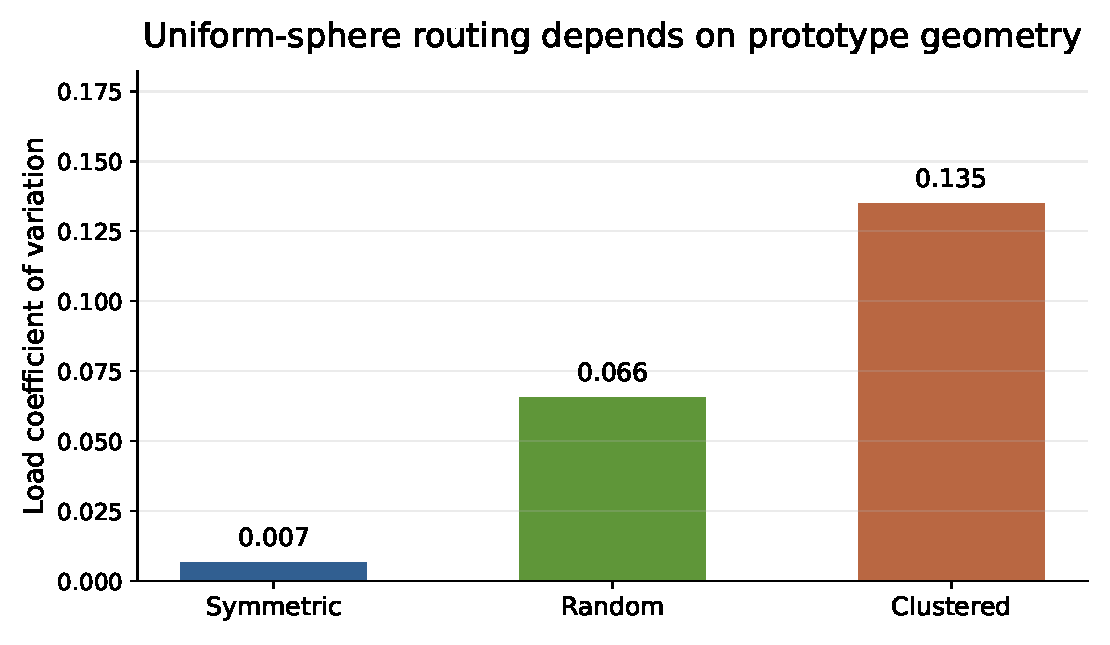
\includegraphics[width=0.72\linewidth]{figures/prototype_geometry_load.pdf}
\caption{Uniform token features do not alone determine expert load.  With the
same feature distribution, prototype geometry changes load variation by more
than an order of magnitude.}
\label{fig:prototype_geometry}
\end{figure}

Table~\ref{tab:uniform_sphere} and Figure~\ref{fig:prototype_geometry} support
the first theoretical condition: load uniformity follows from the combination
of uniform token geometry and well-spread prototypes, not from token-side
uniformity alone.

\subsection{Random centers create a geometric load floor}

The second experiment implements the circular Voronoi model.  For
$E\in\{4,8,16\}$ random centers, we compare the initialization error
$E\max_j |p_j-1/E|$, the sampling error $E\max_j|\widehat p_j-p_j|$, and the
total observed error $E\max_j|\widehat p_j-1/E|$ as token count grows.

\begin{table}[t]
\centering
\caption{Two-dimensional random-center routing.  Sampling error shrinks with
token count, while the initialization error remains fixed for the same random
center realization.}
\label{tab:geometry_floor}
\begin{tabular}{ccccc}
\toprule
Experts & Tokens & Init. error $\downarrow$ & Sampling error $\downarrow$
& Total error $\downarrow$ \\
\midrule
4 & $10^3$ & 0.500 & 0.075 & 0.525 \\
4 & $10^5$ & 0.500 & 0.007 & 0.504 \\
8 & $10^3$ & 1.138 & 0.148 & 1.145 \\
8 & $10^5$ & 1.138 & 0.015 & 1.138 \\
16 & $10^3$ & 1.472 & 0.287 & 1.486 \\
16 & $10^5$ & 1.472 & 0.028 & 1.473 \\
\bottomrule
\end{tabular}
\end{table}

\begin{figure}[t]
\centering
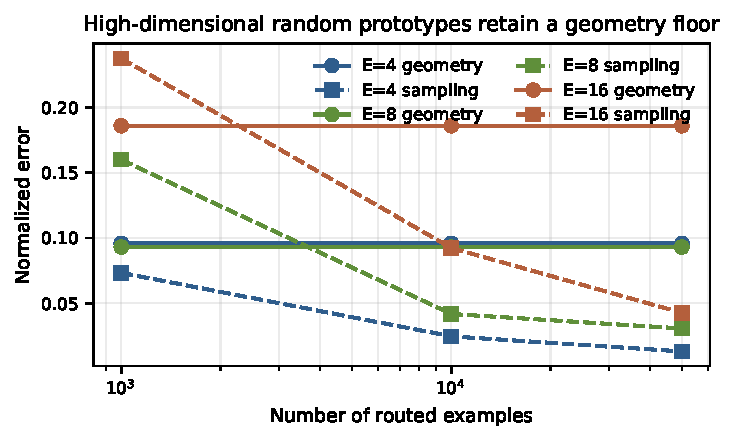
\includegraphics[width=0.76\linewidth]{figures/geometry_floor_sampling.pdf}
\caption{Increasing token count reduces finite-sample noise but leaves the
random-center geometry floor unchanged.  This validates the load decomposition
into prototype-geometry error and sampling error.}
\label{fig:geometry_floor}
\end{figure}

Table~\ref{tab:geometry_floor} and Figure~\ref{fig:geometry_floor} confirm
that random prototypes are not a solution to the single-initialization load
problem.  They are unbiased across draws, but a realized model inherits unequal
cell masses.

\subsection{Spectral prototypes give centers, not balance}

The third experiment constructs synthetic expert matrices whose input-side top
singular directions are prescribed as symmetric, random, or clustered
prototypes.  We compare exact singular-vector prototypes, one-step MPI, five-step
MPI, and random router rows.  The key question is whether high expert alignment
is sufficient for balanced routing.

\begin{table}[t]
\centering
\caption{Spectral prototypes recover expert directions, but load balance still
depends on prototype spread.}
\label{tab:spectral_prototypes}
\begin{tabular}{llccc}
\toprule
Prototype geometry & Router & Alignment $\uparrow$ & Load CV $\downarrow$
& Max/min load $\downarrow$ \\
\midrule
Symmetric & Exact SVD & 1.000 & 0.009 & 1.030 \\
Symmetric & MPI-1 & 0.975 & 0.025 & 1.094 \\
Symmetric & MPI-5 & 1.000 & 0.009 & 1.030 \\
Clustered & Exact SVD & 1.000 & 0.161 & 1.631 \\
Clustered & MPI-1 & 0.977 & 0.195 & 1.788 \\
Clustered & MPI-5 & 1.000 & 0.161 & 1.631 \\
Random rows & No expert alignment & 0.098 & 0.074 & 1.281 \\
\bottomrule
\end{tabular}
\end{table}

\begin{figure}[t]
\centering
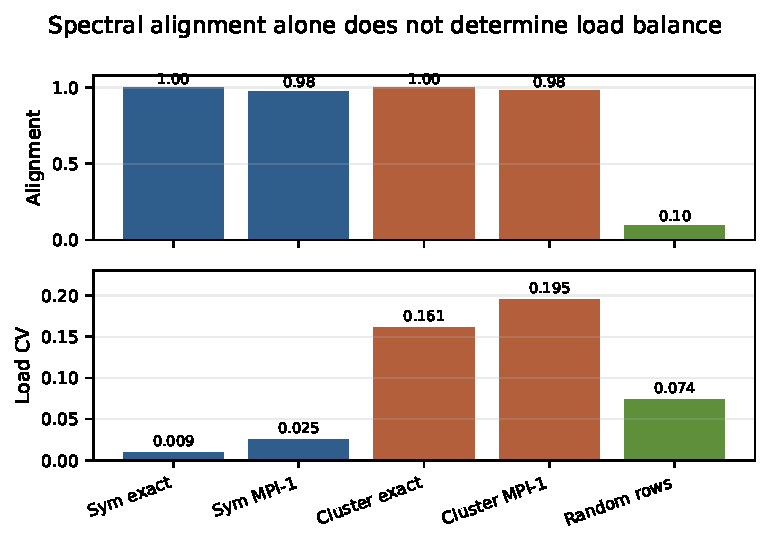
\includegraphics[width=0.78\linewidth]{figures/spectral_alignment_not_balance.pdf}
\caption{High spectral alignment does not imply load balance.  Clustered exact
SVD and MPI rows align with their experts, but their load variation remains
large because the recovered expert directions are not well spread.}
\label{fig:spectral_alignment}
\end{figure}

Table~\ref{tab:spectral_prototypes} and Figure~\ref{fig:spectral_alignment}
support the conditional role of spectral routing.  Expert singular directions
are meaningful centers, and MPI recovers them when the synthetic expert has a
dominant singular direction.  The load theorem still requires the recovered
centers to form a balanced partition of the feature geometry.

\subsection{Capacity-feasible assignment and anisotropic features}

Capacity-feasible assignment, formalized in
Section~\ref{sec:balanced_assignment}, enforces strict empirical load balance
for a finite batch.  In the tested $d=64,E=8,N=4096$ setting, the greedy feasible
assignment reduces LoadCV to $0$ for symmetric, random, and clustered
prototypes.  The mean selected-score drops are small but geometry-dependent:
$0.00059$ for symmetric prototypes, $0.00190$ for random prototypes, and
$0.00538$ for clustered prototypes.  These values are empirical costs of the
greedy feasible assignment, not optimality certificates for the exact assignment
problem.

The final experiment tests frequency-uniform but spectrally anisotropic
features.  Starting from $z\sim\mathrm{Unif}(\mathbb{S}^{63})$, we form
$h=Dz$ with $D=\mathrm{diag}(\alpha,1,\ldots,1)$.  The router prototypes remain
symmetric.  As $\alpha$ grows, the raw representation violates the uniform
spherical assumption.  Whitening and renormalization restore the controlled
geometry.

\begin{table}[t]
\centering
\caption{Anisotropic but frequency-uniform features.  Raw routing becomes
imbalanced as the covariance condition number grows; whitening restores the
uniform-routing regime.}
\label{tab:anisotropy}
\begin{tabular}{ccccc}
\toprule
$\alpha$ & Raw cond. no. $\downarrow$ & Raw LoadCV $\downarrow$
& Whitened cond. no. $\downarrow$ & Whitened LoadCV $\downarrow$ \\
\midrule
1 & 1.10 & 0.008 & 1.00 & 0.005 \\
2 & 4.20 & 0.409 & 1.00 & 0.005 \\
5 & 26.22 & 0.816 & 1.00 & 0.005 \\
10 & 104.88 & 0.972 & 1.00 & 0.005 \\
20 & 419.52 & 1.053 & 1.00 & 0.005 \\
\bottomrule
\end{tabular}
\end{table}

\begin{figure}[t]
\centering
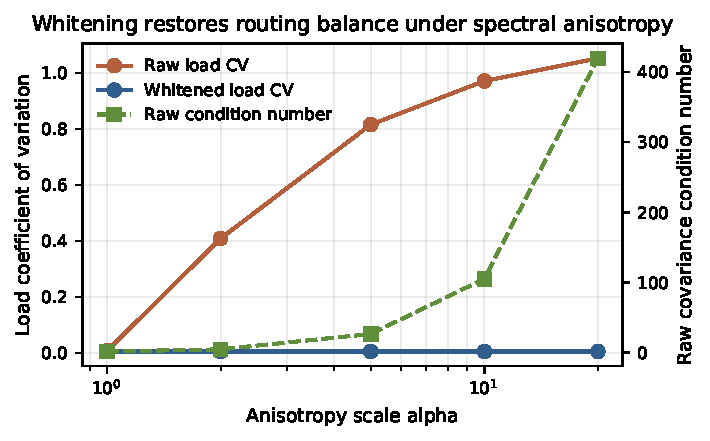
\includegraphics[width=0.76\linewidth]{figures/anisotropy_whitening.pdf}
\caption{Feature frequency can remain uniform while representation geometry
becomes highly anisotropic.  Raw top-1 routing becomes imbalanced under this
anisotropy; whitening returns the feature distribution to the regime described
by the uniform-routing theorem.}
\label{fig:anisotropy}
\end{figure}

Table~\ref{tab:anisotropy} and Figure~\ref{fig:anisotropy} show that the raw
load imbalance tracks spectral anisotropy, while whitening returns both the
condition number and LoadCV to the controlled uniform regime.

\section{Scope and Limitations}

The results establish a controlled static routing statement.  They do not show
that natural language hidden states are geometrically uniform, that learned MoE
experts become semantic specialists, or that a balanced initial assignment is
preserved during training.  Training can move feature centers, router rows, and
expert matrices, so preservation requires additional margin and dynamics
analysis.  The spectral-prototype experiments use synthetic expert matrices with
prescribed singular directions; they test the geometry of spectral centers, not
full-scale language-model transfer.  The balanced-assignment experiment uses a
deterministic capacity-feasible procedure, so its score drops are empirical
costs for that procedure rather than exact optimal costs.

\section{Conclusion}

Uniform feature routing requires both token-side and expert-side structure.
Equal feature frequency is not enough: the route-relevant representation must be
geometrically uniform, or be transformed into such a geometry.  Spectral expert
prototypes are a principled way to obtain router centers, but alignment with
expert singular directions does not guarantee load balance unless those
directions are well spread.  Random prototypes remove bias only across repeated
initializations, not within one realized model.  When exact finite-batch balance
is required, capacity-feasible assignment supplies a separate balancing
constraint and exposes its score cost.  This controlled result is the baseline
case that must be closed before studying nonuniform feature frequencies,
common-direction spectra, training-time preservation, or semantic expert
utility.

\bibliographystyle{iclr2026_conference}
\bibliography{references}

\end{document}
